% DATA 266 Lab 2 combined report. Build on Overleaf, after running build_tables.py.
\documentclass[conference]{IEEEtran}
\usepackage{graphicx,booktabs,cite,tikz,url}
\usetikzlibrary{arrows.meta,positioning}
\title{DATA 266 Lab 2: Multimodal RAG, Diffusion Fine-Tuning and a Multi-Agent Image System}
\author{\IEEEauthorblockN{Kavan Siddesh Kumar and Muhammed Faiq Salman}\IEEEauthorblockA{Pair\_Programming\_Team\_24, San Jos\'e State University}}
\newcommand{\optional}[2]{\IfFileExists{#1}{\input{#1}}{\noindent\textbf{#2}\par}}
\begin{document}
\maketitle
\begin{abstract}
[TO BE WRITTEN LAST, in the team's own words, once results exist.]
\end{abstract}

\section{Part 1: Multimodal RAG}
% We each built a complete Part 1. Both designs are described, then the comparison and the selected system.
% DRAFT written with Claude Code for Kavan's Part 1 system. The brief says "in your own words", so rewrite it before submitting.
\subsection{Architecture}
Our system answers questions over three PDFs, using text, tables and figures \cite{lewis}. Fig.~\ref{fig:p1} shows the flow.
\begin{figure}[!t]
\centering
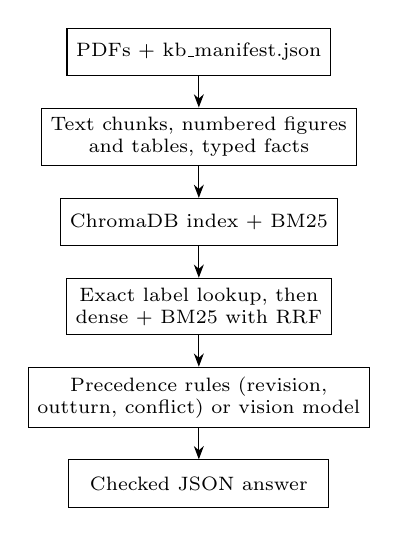
\begin{tikzpicture}[node distance=4mm,box/.style={draw,align=center,font=\scriptsize,minimum width=33mm,minimum height=6mm},>={Stealth}]
\node[box] (pdf) {PDFs + kb\_manifest.json};
\node[box,below=of pdf] (ing) {Text chunks, numbered figures\\and tables, typed facts};
\node[box,below=of ing] (idx) {ChromaDB index + BM25};
\node[box,below=of idx] (ret) {Exact label lookup, then\\dense + BM25 with RRF};
\node[box,below=of ret] (res) {Precedence rules (revision,\\outturn, conflict) or vision model};
\node[box,below=of res] (out) {Checked JSON answer};
\foreach \a/\b in {pdf/ing,ing/idx,idx/ret,ret/res,res/out}{\draw[->] (\a)--(\b);}
\end{tikzpicture}
\caption{Part 1 architecture.}
\label{fig:p1}
\end{figure}

\subsection{Ingestion and retrieval}
We read the PDFs with PyMuPDF. Each chunk keeps its document ID, page and trust level. Every numbered figure and table is saved as an image with its label and caption, so Figure B-5 and Figure B-5 (corrected) stay separate. A local vision model, Qwen2.5-VL-3B, describes each figure, which makes figures searchable as text. Appendix C is indexed with a low trust level, and retrieval filters it out.

Retrieval checks for a named figure or table first, since several charts look almost identical. Otherwise it joins dense and BM25 rankings with reciprocal rank fusion.

\subsection{Grounded answers}
We parsed tables into typed facts (entity, variable, period, value, source, forecast or actual). Plain Python then applies the manifest's precedence rules. We chose this because a small model cannot be trusted to apply them every time. The model reads charts and answers open questions. This code holds no question text or answer values.

\subsection{What worked and what did not}
[PENDING: write this after the GPU run, using real outputs.]

\optional{sections/p1_muhammed.tex}{[PENDING: Muhammed's Part 1 system]}
\optional{sections/p1_eval.tex}{[PENDING: written together at the merge: golden sets, comparison, selection, results, failure and safety analysis]}
\optional{tables/p1.tex}{[PENDING: run build\_tables.py]}

\section{Part 2: Fine-Tuning Diffusion Models}
\optional{sections/p2.tex}{[PENDING: Muhammed's Part 2 section, including the model card summary and Kavan's baseline as reproduction evidence]}
\optional{tables/p2.tex}{[PENDING: run build\_tables.py]}

\section{Part 3: Multimodal Multi-Agent System}
% DRAFT written with Claude Code. The brief says "in your own words", so rewrite it before submitting.
\subsection{Architecture}
Five agents share one typed state object (Fig.~\ref{fig:p3}). The planner routes a request or refuses it. Caption and question requests stop after vision. Other requests continue through the prompt, generation and critique agents, and the critic can send a result back at most twice \cite{madaan}.
\begin{figure}[!t]
\centering
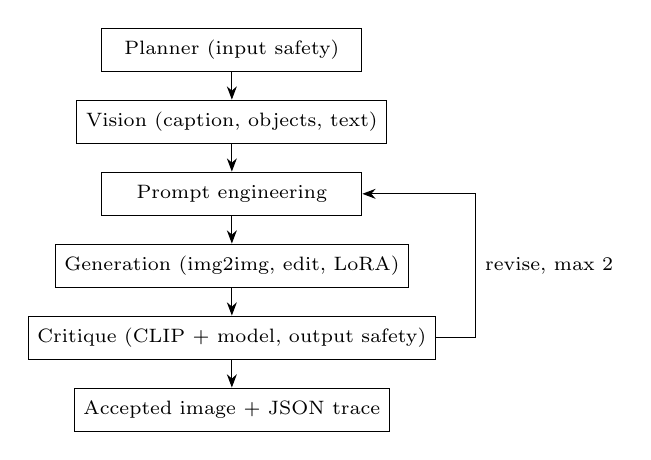
\begin{tikzpicture}[node distance=3.5mm,box/.style={draw,align=center,font=\scriptsize,minimum width=33mm,minimum height=5.5mm},>={Stealth}]
\node[box] (pl) {Planner (input safety)};
\node[box,below=of pl] (vi) {Vision (caption, objects, text)};
\node[box,below=of vi] (pr) {Prompt engineering};
\node[box,below=of pr] (ge) {Generation (img2img, edit, LoRA)};
\node[box,below=of ge] (cr) {Critique (CLIP + model, output safety)};
\node[box,below=of cr] (ou) {Accepted image + JSON trace};
\foreach \a/\b in {pl/vi,vi/pr,pr/ge,ge/cr,cr/ou}{\draw[->] (\a)--(\b);}
\draw[->] (cr.east)--++(5mm,0)|-(pr.east) node[pos=0.25,right,font=\scriptsize]{revise, max 2};
\end{tikzpicture}
\caption{Part 3 architecture.}
\label{fig:p3}
\end{figure}

\subsection{Failure handling}
Broken, empty and unreadable files are caught before any model runs. Every agent runs inside a wrapper that turns an exception into a message and still saves a trace.

\subsection{Safety analysis}
Text in an image is treated as data \cite{greshake}. The planner transcribes visible text, and if it reads like an instruction, generation requests are refused. Caption requests may quote that text as visible text but never act on it. Word patterns catch unsafe requests. The Stable Diffusion safety checker screens outputs, and flagged images never reach the user. [PENDING: results of the 10 red-team cases, with examples, after the GPU run.]

\subsection{System card}
\textbf{Can do:} caption images, answer questions about them, change style, edit, and generate domain-style images with our Part 2 LoRA. \textbf{Known limits:} [PENDING: fill in from observed failures]. Pattern-based checks can miss reworded requests. CLIP is only a rough measure of prompt match. \textbf{Safety measures:} input refusal, hidden-instruction check, output filter, two-revision limit and a JSON trace for every request.

\subsection{What worked and what did not}
[PENDING: write this after the GPU run, using real outputs.]

% p3.tex also needs: Muhammed's baseline as reproduction evidence, and the half-page system card.
\optional{tables/p3.tex}{[PENDING: run build\_tables.py]}

\begin{thebibliography}{00}
\bibitem{lewis} P. Lewis et al., ``Retrieval-augmented generation for knowledge-intensive NLP tasks,'' 2020. arXiv:2005.11401.
\bibitem{faysse} M. Faysse et al., ``ColPali: Efficient document retrieval with vision language models,'' 2024. arXiv:2407.01449.
\bibitem{greshake} K. Greshake et al., ``Not what you've signed up for: Compromising real-world LLM-integrated applications with indirect prompt injection,'' 2023. arXiv:2302.12173.
\bibitem{rombach} R. Rombach et al., ``High-resolution image synthesis with latent diffusion models,'' 2022. arXiv:2112.10752.
\bibitem{hu} E. Hu et al., ``LoRA: Low-rank adaptation of large language models,'' 2021. arXiv:2106.09685.
\bibitem{carlini} N. Carlini et al., ``Extracting training data from diffusion models,'' 2023. arXiv:2301.13188.
\bibitem{yao} S. Yao et al., ``ReAct: Synergizing reasoning and acting in language models,'' 2022. arXiv:2210.03629.
\bibitem{madaan} A. Madaan et al., ``Self-Refine: Iterative refinement with self-feedback,'' 2023. arXiv:2303.17651.
\bibitem{brooks} T. Brooks et al., ``InstructPix2Pix: Learning to follow image editing instructions,'' 2023. arXiv:2211.09800.
\end{thebibliography}
\end{document}
